%%%%%%%%%%%%%%%%%%%%%%%%%%%%%%%%%%%%%%%%%%%%%%%%%%%%%%%%%%%%%%%%%%%%%%%%%%%%%%%%
%2345678901234567890123456789012345678901234567890123456789012345678901234567890
%        1         2         3         4         5         6         7         8

\documentclass[letterpaper, 10 pt, conference]{ieeeconf}  % Comment this line out
                                                          % if you need a4paper
%\documentclass[a4paper, 10pt, conference]{ieeeconf}      % Use this line for a4
                                                          % paper

\IEEEoverridecommandlockouts                              % This command is only
                                                          % needed if you want to
                                                          % use the \thanks command
\overrideIEEEmargins
% See the \addtolength command later in the file to balance the column lengths
% on the last page of the document



% The following packages can be found on http:\\www.ctan.org
%\usepackage{graphics} % for pdf, bitmapped graphics files
\usepackage{epsfig} % for postscript graphics files
%\usepackage{mathptmx} % assumes new font selection scheme installed
%\usepackage{times} % assumes new font selection scheme installed
\usepackage{amsmath} % assumes amsmath package installed
%\usepackage{amssymb}  % assumes amsmath package installed

\title{\LARGE \bf
An Evaluation of Sampling Path Strategies for an Autonomous Underwater Vehicle*
}

%\author{ \parbox{3 in}{\centering Huibert Kwakernaak*
%         \thanks{*Use the $\backslash$thanks command to put information here}\\
%         Faculty of Electrical Engineering, Mathematics and Computer Science\\
%         University of Twente\\
%         7500 AE Enschede, The Netherlands\\
%         {\tt\small h.kwakernaak@autsubmit.com}}
%         \hspace*{ 0.5 in}
%         \parbox{3 in}{ \centering Pradeep Misra**
%         \thanks{**The footnote marks may be inserted manually}\\
%        Department of Electrical Engineering \\
%         Wright State University\\
%         Dayton, OH 45435, USA\\
%         {\tt\small pmisra@cs.wright.edu}}
%}

\author{Andres Mora, Colin Ho, and Srikanth Saripalli% <-this % stops a space
\thanks{*This work was supported in part by NSF grant XYZ}% <-this % stops a space
\thanks{A. Mora, C. Ho, and S. Saripalli are with the School of Earth and Space Exploration, Arizona State University, 550 E. Tyler Mall, Tempe, AZ, USA, 85287
        {\tt\small \{amoravar, srikanth.saripalli, colinho\} at asu.edu}}%
}


\begin{document}



\maketitle
\thispagestyle{empty}
\pagestyle{empty}


%%%%%%%%%%%%%%%%%%%%%%%%%%%%%%%%%%%%%%%%%%%%%%%%%%%%%%%%%%%%%%%%%%%%%%%%%%%%%%%%
\begin{abstract}

A critical problem in planning sampling paths for autonomous underwater vehicles is balancing obtaining an accurate scalar field estimation against efficiently utilizing the stored energy capacity of the sampling vehicle. 
Adaptive sampling approaches can only provide solutions when real-time and a priori environmental data is available. 
Through utilizing a cost-evaluation function to experimentally evaluate various sampling path strategies for a wide range of scalar fields and sampling densities, it is found that a systematic spiral sampling path strategy is optimal for high-variance scalar fields for all sampling densities and low-variance scalar fields when sampling is sparse. 
The random spiral sampling path strategy is found to be optimal for low-variance scalar fields when sampling is dense.

\end{abstract}


%%%%%%%%%%%%%%%%%%%%%%%%%%%%%%%%%%%%%%%%%%%%%%%%%%%%%%%%%%%%%%%%%%%%%%%%%%%%%%%%
\section{INTRODUCTION}
Autonomous underwater vehicles (AUV) are mobile robotic platforms that are utilized for environmental sampling, sensing and are capable of operating in a multitude of underwater aquatic environments \cite{forrest:investigation}.
In research they are commonly used to carry hydrological, geophysical, and/or biological sensor payloads that are used to gather remote and in-situ data to aid the study of open and closed aquatic bodies \cite{stoker:exploration}, \cite{german:hydro}.

An autonomous underwater vehicle is generally described as being capable of operation without any human controller; thus it must be able to traverse the aquatic environment on a desired path through autonomous navigation and control \cite{kumagai:newAUV}. 
An example of an autonomous underwater vehicle is the one used in this paper to collect the data that was then processed to generate scalar fields (see Figure \ref{fig:iverAtPleasant}).

The goal of environmental sampling and sensing is to generate an accurate estimate of the underlying scalar field(s) over an area of interest. 
An estimate is generated by interpolating the sensing data collected over the area being studied. 
In the case of aquatic environments, a mobile vehicle can be used to collect the necessary sensing data. 
However the sensing platform is limited in range by the amount of stored energy it carries aboard. 
The problem of environmental sensing then becomes determining how one obtains an accurate estimation of the scalar field of interest while being constrained by the amount of stored energy the vehicle can utilize in order to sample the scalar field.

\begin{figure}[htp]
	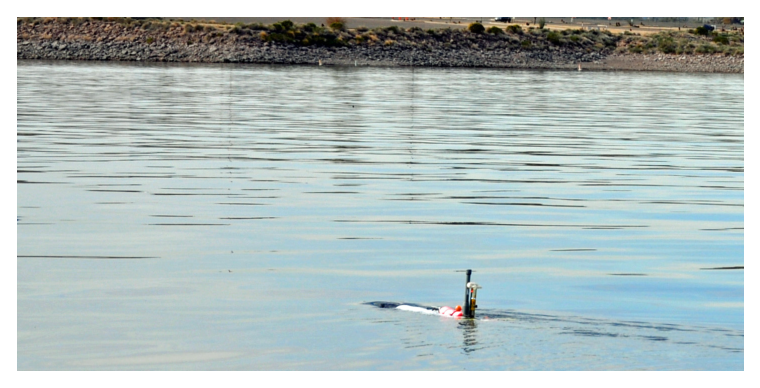
\includegraphics[width=\columnwidth, scale= 0.6]{figs/iverAtPleasant}
	\caption{Modified OceanServer IVER2 AUV at Lake Pleasant.}
	\label{fig:iverAtPleasant}
\end{figure} 

The purpose of this paper is to experimentally evaluate sampling strategies based upon estimation accuracy and energy consumption. 
This evaluation is conducted with a cost-evaluation function that considers multiple parameters, and can assign priorities to each factor. 
The evaluation takes into account real world and simulated isotropic, anisotropic scalar fields, as well as varying sampling densities to determine which sampling strategy is optimal for different scalar field types, for a range of sampling densities. 
The sampling path strategies evaluated in this study were systematic and stratified random sampling distributions with spiral and lawn mower sampling paths. 

Through utilizing the cost-evaluation function, it is found that the systematic spiral sampling path strategy best optimizes the energy consumption with the scalar reconstruction error compared to the other sampling path strategies evaluated. 
Additionally, it is found that the systematic spiral path consumes the least amount of energy out of the sampling path strategies evaluated.


\section{RELATED WORK}
In the fields of robotics, hydrology, geology, and geostatistical sciences, optimal sample collection and path planning are an active area of research \cite{mcbratney:exploration}. 
There is much prior and current work ongoing in the domain of path planning and sampling optimization for autonomous vehicles. 
For example, adaptive sampling algorithms have been developed that can direct the path of single or multiple autonomous underwater vehicles in towards locations of high probable data yield \cite{popa:adaptive}, and can be used in conjunction with existing sensor networks \cite{zhang:adaptive}. 
Additionally, energy optimal paths can be computed based upon known and sensed external variables such as ocean currents \cite{witt:go}-\cite{smith:autonomous}, and static or dynamic obstacles \cite{caldwell:reconfiguring}.

However all of these planning schemes require a priori knowledge of the environment or real time sensing and data feedback. 
There are many AUV deployments scenarios where there is a lack of a priori data on the environment, and the AUV is equipped with sensors that do not provide real time data (such as taking physical water samples) \cite{stoker:exploration}. 
Therefore, in many real world deployments, the paths chosen are often simple lawnmower patterns that may or may not be optimal for the situation they are being utilized \cite{forrest:investigation}, \cite{stoker:exploration}. 
The evaluation conducted in this paper is targeted at looking at autonomous underwater vehicle path planning from an experimental field scientist�s data sampling perspective. 
The goal is to comparatively evaluate various sampling path strategies using a cost-evaluation function that can optimize multiple parameters. 
These results from this evaluation will aid choosing the best sampling path strategy for unknown scalar fields, with no real time data feedback.


\section{EXPERIMENTAL APPROACH}
The evaluation consisted of conducting AUV sampling paths over various scalar fields to generate estimations of those scalar fields, and the energy consumption of the sampling path taken. 
Each of the simulated sampling paths and their corresponding scalar field estimation and energy consumption are then used as inputs for a cost-evaluation function that is used to comparatively determine the optimal sampling path.

\subsection{Assumptions} 
The following assumptions are made:
\begin{itemize}
    \item[1)] The simulated AUV travels at a constant velocity and is capable of navigating to the desired sampling locations.
    \item[2)] The vehicle�s total energy consumption is based upon the total distance it travels, and the total angle it turns.
    \item[3)] The underlying scalar field being sampled has little or no temporal variation while being sampled.
    \item[4)] There is no real-time access to the sampled data; the samples can only be accessed offline.
  \end{itemize}

\subsection{Sampling Strategies}
The two main sampling strategy types that are evaluated are systematic sampling, and stratified random sampling.  
Systematic sampling is defined as sampling from an area of interest at regularly spaced intervals. 
Prior research has shown that having equilateral sampling grids is only optimal when the scalar field variation is isotropic \cite{mcbratney:exploration}. 
Therefore stratified random sampling was chosen as an additional sampling method to be comparatively evaluated. 
Stratified random sampling is conducted by splitting the desired sampling area into grid of equal sized sub-areas, in which samples are chosen from a random location in each sub-area. 
Stratified random sampling often produces a weighted mean with less variability than a standard random sampling. 
For each type of sampling strategy, lawn mower and spiral path patterns are evaluated. 
Both are simple path patterns which are commonly used for surveying. Example paths of the four sampling strategies are shown in Figure 2.

\subsection{Underlying Scalar Field Data}
The underlying scalar field was represented with both real world and simulated data. 
The goal was to utilize enough scalar field data to be representative of many scalar field distributions commonly seen in real world data sets. 
Thus, six different underlying scalar fields were generated and collected for the purposes of this evaluation and are shown in Fig. 3. 
The data sets derived from real world data consisted of a turbidity data set representing multi-modal data, a chlorophyll data set representing high anisotropy and variance, and a blue green algae cell count data set representing moderate anisotropy data with a high degree of spatial variance. 
The first simulated data set was a linearly varying distribution representing isotropic data. 
The second simulated data set was a normal distribution that represented moderately anisotropic data. 
The third and final simulated data set was a bi-modal normal distribution that represented moderate-variance anisotropic data.



\section{EVALUATION METHODS}

\subsection{Estimation Evaluation}

Once a sampling path has been generated, it is then used to sample the underlying scalar field. 
With those samples, an estimation of the underlying scalar field is generated through ordinary Kriging. 
Kriging is a form of linear least squares estimation that interpolates the value of a location upon a scalar field from known values at nearby locations, which in this case are the sampled locations \cite{delhomme:kriging}.
Ordinary Kriging is a specific type of Kriging that assumes that the experimental variogram can be constructed, and that the mean of the scalar field being estimated is unknown but constant. 
Z represents the underlying scalar field, thus the Kriging estimation of the scalar field at any location is the weighted average of observed values. 
This is represented through the following equation (\ref{eq:scalarField}). 

\begin{equation}
z(x_0) = \Sigma^n_{i=1} w_i z(x_i)
\label{eq:scalarField}
\end{equation}


The estimation variance of z(xo) is given by

\begin{equation}
\sigma^2_k = 2 \Sigma^n_{i=1} w_i \gamma(x_i, x_0) - \Sigma^n_{j=1} w_i w_j \gamma(x_i, x_j)
\label{eq:estimVar}
\end{equation}

where $\gamma(x_i, x_0)$ is the variogram of $x_i$ and $x_0$. 
The weights $w_i(x)$ are chosen such that tehy fulfull the unbiasedness condition (they all sum to $1$), and also minimize the estimation variance.
Thus, the weights are determined through the equation (\ref{eq:weights})

\begin{equation}
\Sigma^n_{j=1} w_j \gamma(x_i, x_j) + \psi = \gamma(x_i, x_0)
\label{eq:weights}
\end{equation}

where $\gamma$ is the Lagrance parameter associated with the minimization.
Once the Kriging estimation was generated, it accuracy is evaluated through the computation of its integrated mean square error (IMSE) with respect to the underlying scalar field.


\subsection{Energy Consumption Evaluation}
In order to improve the simple energy consumption model used in previous studies \cite{ho:where}, an estimation of the dynamical model of the robot based on the selection of two known inputs and one output from the data acquired was used.
The two inputs of the estimation were the velocity and the heading of the vehicle measured by the on-board GPS.
The output selected for the estimation of our model was the total power consumed by the vehicle during the sampling mission.
The estimation consisted of first calculating the state-space model using a sub-space method and later on refining the model by computing the prediction error estimate of the state-space model.

With this estimated model, it is not required to assume that the vehicle is travelling straight at a constant velocity, thus there is no restriction with respect to the rate at which the vehicle consumes its stored energy.
An increase in the energy consumed by the vehicle while it turns may be nominal or significant, depending on the design of the vehicle.
The estimated model incorporates the possible effect in the increment in energy consumption a turning maneuver may represent by including the changes in the orientation of the vehicle.
The velocity of the vehicle (in knots), its heading (in degrees) and the corresponding power consumption (in Watts) measured by the instruments on-board are presented in Figuer \ref{fig:inputsVsOutput}.

\begin{figure}
	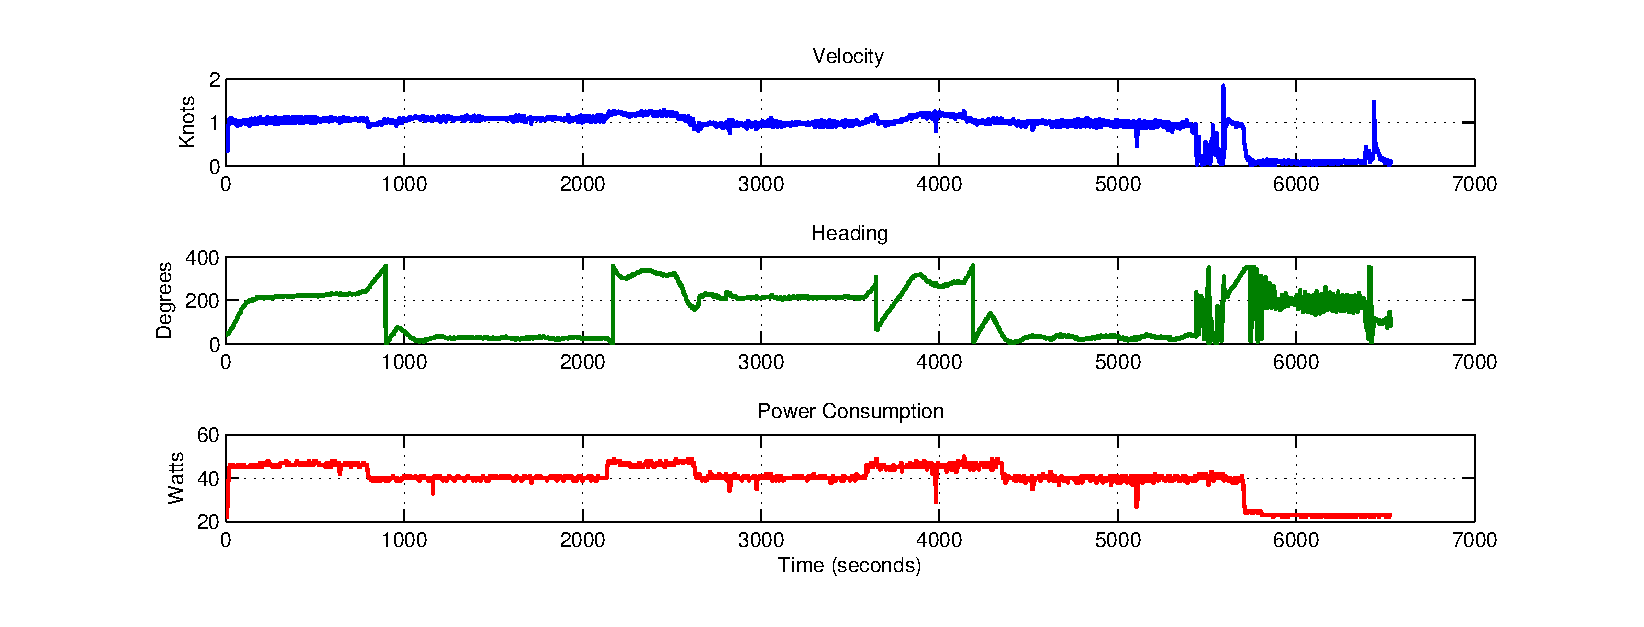
\includegraphics[width=\columnwidth, scale= 1.0]{figs/inputsVsOutput.eps}
	\caption{Velocity, heading and power consumption used to estimate the vehicle's dynamical model.}
	\label{fig:inputsVsOutput}
\end{figure}

In order to estimate and validate the model, the estimation is based on half of the entire data set and it is later validated using the remaining half of the data set acquired by the vehicle's instruments (GPS, XXYY, etc.). 


The resulting dynamic model obtain from the estimation follows the standard state-space model convention as presented by equation \ref{eq:dynModel_1}:

\begin{equation}
 \left\{\begin{aligned}
        x(t + Ts) &= Ax(t) + Bu(t) + Ke(t) \\
        y(t) &= Cx(t) + Du(t) + e(t)
       \end{aligned}
       \right.
\label{eq:dynModel_1}
\end{equation}

where 
$ 
A = 
\bigl[
\begin{smallmatrix}
	0.99495		&	-0.069517 \\
	 -0.0032466	&	0.86892
\end{smallmatrix} 
\bigr]
$,
$ 
B = 
\bigl[
\begin{smallmatrix}
	0.021859	&	1.0813e^{-5} \\
    -0.039972	&	1.9386e^{-5}
\end{smallmatrix} 
\bigr]
$,
$ 
C = 
\bigl[
\begin{smallmatrix}
	126.37	& 6.4396
\end{smallmatrix} 
\bigr]
$,
$ 
D = 
\bigl[
\begin{smallmatrix}
	0 & 0
\end{smallmatrix} 
\bigr]
$, 
$ 
K = 
\bigl[
\begin{smallmatrix}
	0.0070135	\\
    0.0090162
\end{smallmatrix} 
\bigr]
$, and 
$ 
x(0) = 
\bigl[
\begin{smallmatrix}
	-0.14306\\
    -0.36083
\end{smallmatrix} 
\bigr]
$.
The data acquisition frequency was set to $2Hz$. 

The resulting power based on the estimated dynamical model is compared against the half of the data set used to validate the model as shown in Figure \ref{fig:estVsMeaPwr}. 

\begin{figure}[htp]
	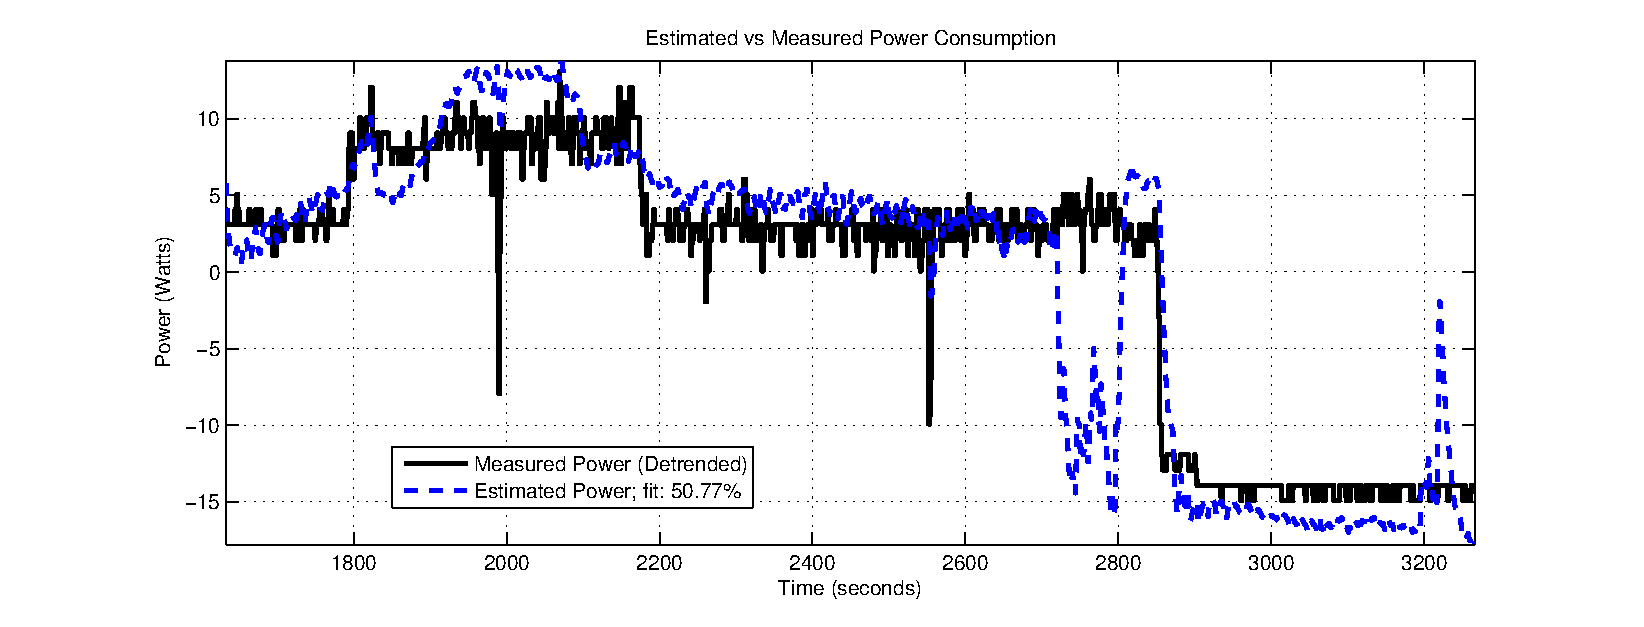
\includegraphics[width=\columnwidth, scale= 1.0]{figs/estimatedVsMeasuredPower}
	\caption{Estimated vs Measured Power Consumption.}
	\label{fig:estVsMeaPwr}
\end{figure} 

% The energy consumed by the vehicle travelling along the sampling path was computed through the use of a simple energy consumption model. 
% The model has two input parameters; the distance travelled, and the total angle turned. 
% Since it is assumed that the vehicle is travelling straight at a constant velocity, it is extrapolated that the vehicle consumes its stored energy at a constant rate.
% An autonomous underwater vehicle may also experience in increase in energy consumption while turning. 
% This additional increase may be nominal or significant, depending on the design of the vehicle. 
% Therefore the model takes the additional energy consumption while turning into consideration through the use of a constant multiplier for the total turn angle. 
% The energy consumption equation is modeled through the following equation Figure 
% 
% 
% 
% \begin{equation}
% E(d, \theta) = d + k_\theta
% \label{eq:energyConsumption}
% \end{equation}
% 
% For this equation, $d$ and $\theta$ respectively represent the total distance of the sampling path, and the cumulative turn angle. 
% The constant $k_\theta$ is a constant multiplier that represents the increase in energy consumption while turning for a vehicle. 
% This weight is better understood through the following relation.
% 
% \begin{equation}
% k_\theta = \frac{d_t}{90^o}
% \label{eq:weightK}
% \end{equation}
% 
% This relation defined as such; for each right angle turn taken, an additional energy penalty of travelling a straight distance $d_t$ is added.

\subsection{Cost-Evaluation Function}
The cost-evaluation function is a general evaluation method that allows for quantitative comparative analysis for multiple input parameters. 
It normalizes and then assigns each input parameter a weight, allowing for the function to prioritize each parameter in respect to one another. 
These weights must all sum to one. 
In the case of this evaluation, we are investigating which sampling strategy is optimal for both estimation error and energy consumption. 
Therefore the parameters that were selected to be inputs for the cost-evaluation function were the total distance travelled  $d$, the total energy consumed E, and the IMSE for the specific sampling path taken $\epsilon$.  
Our proposed cost-evaluation function is as follows,

\begin{equation}
E(p) = \Sigma_{i=p} W_d N_d d_i + W_E N_E E_i + W_\epsilon N_\epsilon \epsilon_i
\label{eq:costFunction}
\end{equation}

where $W_d$, $W_E$, and $W_\epsilon$, are the weighted factors that provide specific priorities between the total distance travelled, the total energy consumed, and the IMSE for the sampling path taken.  
$N_d$, $N_E$, and $N_\epsilon$ are normalization factors assigned constant values to normalize each of their corresponding parameters and eliminate their dimensions.

\section{EXPERIMENTAL RESULTS AND DISCUSSION}

\subsection{Underlying Scalar Field Data Generation}
The six different scalar fields used in this evaluation were either generated from simulated equations, or from a real world dataset. 
The isotropic scalar field used for this evaluation was generated by the following equation.

\begin{equation}
I(x, y) = \frac{x+y}{0.1} + 20
\label{eq:isoScalarField}
\end{equation}

The first simulated anisotropic scalar field was generated by using a standard normal distribution and then scaling it by a factor of 50 and offseting by +20. 
The multi-modal anisotropic field was generated by simply adding together two equally scaled inverted normal distributions with differing $x-y$ locations for their means. 
The real world dataset used for generating the turbidity, chlorophyll and blue green algae scalar fields was created by sampling a local freshwater lake with an autonomous underwater vehicle carrying a water quality monitoring sonde. 
The contiguous underlying scalar field was then generated by interpolating the samples using ordinary kriging.

The AUV to used to collect the samples was a heavily modified OceanServer IVER2 platform, which carries a YSI 6600V2 water quality monitoring sonde. 
The sonde sampled the in-situ turbidity, cholorophyll, and blue green algae, among a variety of other measurements.

All of the samples were taken at Lake Pleasant, a large freshwater reservoir in Arizona. 
The approximate coordinates of the sampling location are $33o 51� 55.66�$ N and $112o 17�45.01�$ W. The sampling locations are shown in Fig. 3. 
The AUV collected 2258 samples over an area of approximately 70[m] x 100[m]. A subset of the samples from 30-70[m] northing and 30-70[m] easting was selected, since it was the region containing the highest density of samples.

\subsection{Estimation Error Computation}
To compute the estimation error, an estimate of the underlying scalar field was first generated for each of the sampling strategy types. 
These estimates were generated across varying sampling grid sizes in order to characterize a range of sampling densities from low to high. 
The sampling grid dimensions and total sample size are listed in Table I.

The IMSE for each of the stratified random sampling strategy based estimations was the average of fifteen iterations, in order to generate a stable value. 
The systematic sampling estimation was iterated five times at five separate evenly distributed path seeding locations to remove biasing in error results. 
These seeding locations are shown in Fig. 4. 

\subsection{Estimation Error Result}
The IMSE error for each of the scalar varying from low (20 samples), moderate (56 samples) and high (120 samples) sampling density are displayed alongside one another in the Table II on the following page.

Through looking at the IMSE versus number of sample plots for the various underlying scalar fields, a number of correlations are apparent. 
Firstly, both strategies demonstrate a reduction in IMSE as the number of samples increases, as one would expect. 
Additionally, it is found that the systematic sampling strategy minimizes error for the real world data sets across all sampling densities. 
The stratified random sampling strategy minimizes error for the low variance isotropic and anisotropic 2 data sets. 
Finally, for the anisotropic 1 data set, the systematic sampling strategy significantly minimizes error for low sampling densities, and the stratified random sampling strategy minimizes error for moderate and high sampling densities.

\subsection{Energy Consumption Computation}
The energy consumption of each of the sampling path patterns was computed using (4). 
First, the distance and total angle turned was computed for each of the sampling path types through the range of sampling densities shown in Table I.  
For each of the stratified random sampling paths, the total distance travelled and total cumulative angle turned was computed as the averages of 50 iterations of each sample grid size. 
Finally (4) was applied using $k_\theta$ values from a range of 0 to 2. 
This range characterizes vehicles for which a $90^o$ turn correlates to consuming the energy equivalent to travelling an additional distance of 0[m] to 2[m].

\subsection{Energy Consumption Results}
The average total energy consumption versus the $k_\theta$ for each of the sampling path strategies is shown in Fig. 9. 
The resulting total energy versus $k_\theta$ plots were then fitted to linear equations to quantify their relationship. 
The resulting energy consumption model equations for each of the sampling path strategies are shown below in Table III.

It is shown in the energy consumption model equations, that the even spiral sampling path strategy is the most energy efficient, and through viewing Figure 9, it is easily apparent.

\subsection{Cost-Evaluation Computation}

The cost-evaluation function was computed with the all the weighted factors set equal to $1/3$, thus weighting all of the evaluation parameters equally. 
To compute the energy for each sampling path, $k_\theta$ was set to 0.1. 
The function was applied to each of the sampling strategies for all the underlying scalar fields, at 20, 56, and 120 samples. 
This was done such that a comparative analysis of each of the sampling strategies at low, moderate and high sampling densities could be conducted. 

\subsection{Cost-Evaluation Results}
The results of the cost-evaluation are listed in Table IV. 
For a low sampling density the systematic spiral sampling method is optimal for all of the data sets except for the isotropic scalar field. 
For a moderate sampling density the systematic spiral strategy is optimal for the anisotropic 1, turbidity, and chlorophyll scalar fields. 
The random lawnmower and random spiral strategies are optimal for the anisotropic 2 and isotropic scalar fields respectively. 
Finally, for a high sample density the random spiral strategy is optimal for the isotropic and both of the anisotropic scalar fields. 
The systematic spiral strategy was found to be optimal for the turbidity, cholorophyll and blue green algae scalar fields. 
The strategy that was optimal for the most types of scalar fields and densities was found to be the systematic spiral strategy. 
In general, a spiral path strategy was found to be the optimal in almost all of the cases. 

\subsection{Discussion of Results}
The results from this cost-evaluation are specific to the weights given to the cost-evaluation function. 
However these results do provide insight into which sampling strategies are optimal for different types of scalar fields, given the assumption that distance travelled, total energy consumption and IMSE are considered equal factors in optimality. 

For isotropic scalar fields, the random spiral sampling strategy was found to be the optimal sampling strategy for all sampling densities. 

It was found that in low variance scalar fields, such as the single/multi-modal anisotropic scalar fields used in this evaluation, the systematic spiral strategy is optimal for coarse sampling densities, and the random spiral strategy is optimal for high sampling densities.

In high variance scalar fields such as the turbidity, chlorophyll and blue green algae data sets, the systematic spiral strategy was optimal for almost every case.


\section{CONCLUSIONS}

We experimentally evaluated four different sampling strategies through a cost-evaluation function.
Assuming that optimality was defined as minimizing the total path distance, the total energy consumed, and the IMSE, it was found that the systematic spiral sampling strategy was the most optimal strategy overall. 
Thus if one were given the task to choose a sampling strategy given no a priori knowledge of the underlying scalar field and no access to the sampled data in real time, the best sampling strategy to choose would be a systematic spiral path, rather than a standard systematic lawnmower path. 
It was also demonstrated that the cost-evaluation function is a useful tool that can be used to quantify overall optimality for multiple sampling strategy parameters.

In the future we plan on further experimentally validating the results of this evaluation. 
Additionally, the cost-evaluation function can be utilized to create an online path optimization planner that chooses path options in real time.

\addtolength{\textheight}{-12cm}   % This command serves to balance the column lengths
                                  % on the last page of the document manually. It shortens
                                  % the textheight of the last page by a suitable amount.
                                  % This command does not take effect until the next page
                                  % so it should come on the page before the last. Make
                                  % sure that you do not shorten the textheight too much.

%%%%%%%%%%%%%%%%%%%%%%%%%%%%%%%%%%%%%%%%%%%%%%%%%%%%%%%%%%%%%%%%%%%%%%%%%%%%%%%%



%%%%%%%%%%%%%%%%%%%%%%%%%%%%%%%%%%%%%%%%%%%%%%%%%%%%%%%%%%%%%%%%%%%%%%%%%%%%%%%%



%%%%%%%%%%%%%%%%%%%%%%%%%%%%%%%%%%%%%%%%%%%%%%%%%%%%%%%%%%%%%%%%%%%%%%%%%%%%%%%%
% \section*{APPENDIX}
% 
% Appendixes should appear before the acknowledgment.

% \section*{ACKNOWLEDGMENT}
% The authors would like to acknowledge the following individuals for their support and help: Alexander Kafka, Brance Hudzietz, and Yucong Lin.



%%%%%%%%%%%%%%%%%%%%%%%%%%%%%%%%%%%%%%%%%%%%%%%%%%%%%%%%%%%%%%%%%%%%%%%%%%%%%%%%


\bibliographystyle{abbrv}
\bibliography{moraIROS2012} 

% \begin{thebibliography}{99}
% \bibitem{c1} A. L. Forrest, H. Bohm, B.  Laval, E. Magnusson, R. Yeo, M. J.  Doble, ``Investigation of under-ice thermal structure: small AUV deployment in Pavilion Lake, BC, Canada,'' OCEANS 2007 , pp.1-9, Sept. 29 2007-Oct. 4 2007.
% 
% \bibitem{c2} C. R . Stoker, D. Barch, J. Farmer, M.  Flagg, T.  Healy, T. Tengdin, H. Thomas, K. Schwer, D. Stakes, ``Exploration of Mono Lake with an ROV: a prototype experiment for the MAPS AUV program,'' Autonomous Underwater Vehicle Technology, 1996. AUV '96., Proceedings of the 1996 Symposium on, pp.33-40, 2-6 Jun 1996.
% 
% \bibitem{c3} M. Kumagai, T. Ura, Y. Kuroda, R. Walker, ``New AUV designed for lake environment monitoring,'' Underwater Technology, 2000. UT 00. Proceedings of the 2000 International Symposium on , vol., no., pp.78-83, 2000.
% 
% \bibitem{c4} A. B. McBratney, R. Webster, T. M. Burgess, ``The design of optimal sampling schemes for local estimation and mapping of of regionalized variables I: Theory and method," Computers and Geosciences, Volume 7, Issue 4, 1981, pp. 331-334.
% 
% \bibitem{c5} D. O. Popa, A. C. Sanderson, R. J. Komerska, S. S. Mupparapu, D. R. Blidberg, S. G. Chappel, ``Adaptive sampling algorithms for multiple autonomous underwater vehicles,'' Autonomous Underwater Vehicles, 2004 IEEE/OES , vol., no., pp. 108- 118, 17-18 June 2004. 
% 
% \bibitem{c6} B. Zhang, G. S. Sukhatme, ``Adaptive Sampling for Estimating a Scalar Field using a Robotic Boat and a Sensor Network,'' Robotics and Automation, 2007 IEEE International Conference on , vol., no., pp.3673-3680, 10-14 April 2007.
% 
% \bibitem{c7} J. Witt, M. Dunbabin, ``Go with the Flow: Optimal AUV Path Planning in Coastal Environments,'' Australian Conference on Robotics and Automation, 2008.
% 
% \bibitem{c8} R. N. Smith, A. Pereira, Yi Chao, P. P. Li, D. A. Caron, B. H. Jones, G. S. Sukhatme, ``Autonomous Underwater Vehicle trajectory design coupled with predictive ocean models: A case study,'' Robotics and Automation (ICRA), 2010 IEEE International Conference on, pp.4770-4777, 3-7 May 2010.
% 
% \bibitem{c9} C. V. Caldwell, D. D. Dunlap, E. G. Collins, ``Motion planning for an autonomous Underwater Vehicle via Sampling Based Model Predictive Control,'' OCEANS 2010, pp.1-6, 20-23 Sept. 2010.
% 
% \bibitem{c10} J. P. Delhomme, Kriging in the hydrosciences, Advances in Water Resources, vol. 1, no. 5, September 1978, pp. 251-266.
%
%\end{thebibliography}




\end{document}
